% Straight up stealing preamble from Eli Holmes 
%%%%%%%%%%%%%%%%%%%%%%%%%%%%%%%%%%%%%%START PREAMBLE THAT IS THE SAME FOR ALL EXAMPLES
\documentclass{article}

%Required: You must have these
\usepackage{Sweave}
\usepackage{graphicx}
\usepackage{tabularx}
\usepackage{hyperref}


%Strongly recommended
  %put your figures in one place
% \SweaveOpts{prefix.string=/Users/Lizzie/Documents/git/projects/meta_ep2/radcliffe/sweave/figures, eps=FALSE} 
%you'll want these for pretty captioning
\usepackage[small]{caption}
\setkeys{Gin}{width=0.8\textwidth}  %make the figs 50 perc textwidth
\setlength{\captionmargin}{30pt}
\setlength{\abovecaptionskip}{0pt}
\setlength{\belowcaptionskip}{10pt}
% manual for caption  http://www.dd.chalmers.se/latex/Docs/PDF/caption.pdf

%Optional: I like to muck with my margins and spacing in ways that LaTeX frowns on
%Here's how to do that
 \topmargin -1.5cm        
 \oddsidemargin -0.04cm   
 \evensidemargin -0.04cm  % same as oddsidemargin but for left-hand pages
 \textwidth 16.59cm
 \textheight 21.94cm 
 %\pagestyle{empty}       % Uncomment if don't want page numbers
 \parskip 7.2pt           % sets spacing between paragraphs
 %\renewcommand{\baselinestretch}{1.5} 	% Uncomment for 1.5 spacing between lines
\parindent 0pt		  % sets leading space for paragraphs
\usepackage{setspace}
%\doublespacing

%Optional: I like fancy headers
\usepackage{fancyhdr}
\pagestyle{fancy}
\fancyhead[LO]{Meta-analysis, episode 2}
\fancyhead[RO]{2016}
 
%%%%%%%%%%%%%%%%%%%%%%%%%%%%%%%%%%%%%%END PREAMBLE THAT IS THE SAME FOR ALL EXAMPLES

%Start of the document
\begin{document}
\Sconcordance{concordance:meta_ep2_data.tex:meta_ep2_data.Rnw:%
1 67 1 1 4 1 7 2 1 1 2 13 0 1 2 4 1 1 2 13 0 1 2 2 1 1 2 9 0 2 2 22 0 1 2 2 1 1 %
12 1 2 5 1 1 2 1 0 2 1 5 0 1 1 6 0 1 2 2 1 1 2 27 0 1 2 1 1}

% \SweaveOpts{concordance=TRUE}
% \bibliographystyle{/Users/Lizzie/Documents/EndnoteRelated/Bibtex/styles/nature.bst}

\title{Data Overview: \\ \\ Predicting Future Springs} % Reconciling Experimental and Observational Approaches for Climate Change Impacts
\author{A. K. Ettinger, E. M. Wolkovich \& the Predicting Future Springs Working Group}
%\date{\today}
\maketitle  %put the fancy title on
%\tableofcontents      %add a table of contents
%\clearpage
%%%%%%%%%%%%%%%%%%%%%%%%%%%%%%%%%%%%%%%%%%%%%%%%%%%
\renewcommand{\thetable}{S\arabic{table}}
\renewcommand{\thefigure}{S\arabic{figure}}
\renewcommand{\labelitemi}{$-$}

%%%%%%%%%%%%%%%% Here we go, boys and girls %%%%%%
\section {Overview of the phenological data}

There are two main files with the phenological data. They can both be downloaded from \url{https://github.com/AileneKane/radcliffe}.

\subsection{Experimental data}



We'll walk through the experimental datafile first. Repeat what's below for the observational data ....

\begin{Schunk}
\begin{Sinput}
> head(expdata)
\end{Sinput}
\begin{Soutput}
     site plot event year genus species doy
1 marchin    1   bbd 2011  Acer  rubrum  88
2 marchin    1   bbd 2011  Acer  rubrum  83
3 marchin    1   bbd 2011  Acer  rubrum  96
4 marchin    1   bbd 2011  Acer  rubrum  79
5 marchin    1   bbd 2011  Acer  rubrum  83
6 marchin    1   bbd 2011  Acer  rubrum  80
\end{Soutput}
\end{Schunk}

\subsection{Observational data}

Next, the observational data. Here we explain what each column means ....

\begin{Schunk}
\begin{Sinput}
> head(obsdata)
\end{Sinput}
\begin{Soutput}
    site plot event year doy       date genus   species scrub varetc cult
1 fitter <NA>   ffd 1954 130 1954-05-10  Acer campestre     0     NA   NA
2 fitter <NA>   ffd 1955 131 1955-05-11  Acer campestre     0     NA   NA
3 fitter <NA>   ffd 1956 137 1956-05-16  Acer campestre     0     NA   NA
4 fitter <NA>   ffd 1957 121 1957-05-01  Acer campestre     0     NA   NA
5 fitter <NA>   ffd 1958 128 1958-05-08  Acer campestre     0     NA   NA
6 fitter <NA>   ffd 1959 129 1959-05-09  Acer campestre     0     NA   NA
\end{Soutput}
\end{Schunk}

Then we could discuss the sites, and the phenological events ...

\begin{Schunk}
\begin{Sinput}
> unique(obsdata$site)
\end{Sinput}
\begin{Soutput}
 [1] fitter   harvard  hubbard  konza    niwot    mikesell concord  mohonk   marsham 
[10] fargo    washdc   bolmgren gothic   uwm      rousi   
15 Levels: bolmgren concord fargo fitter gothic harvard hubbard konza ... washdc
\end{Soutput}
\end{Schunk}

\begin{Schunk}
\begin{Sinput}
> table(obsdata$site, obsdata$event)
\end{Sinput}
\begin{Soutput}
              bbd    ffd    fld L75mdoy L95mdoy    lod    lud
  bolmgren      0   1622      0       0       0      0      0
  concord       0   9320      0       0       0      0      0
  fargo         0   4725      0       0       0      0      0
  fitter        0  13721      0       0       0      0      0
  gothic        0 162352      0       0       0      0      0
  harvard     483    284      0       0       0      0      0
  hubbard      72      0      0       0       0     72      0
  konza         0   3403      0       0       0      0      0
  marsham       0   2131    660       0       0      0      0
  mikesell    445      0      0       0       0    549    554
  mohonk        0    673      0       0       0      0      0
  niwot       648    371      0       0       0      0      0
  rousi      1021    147      0       0       0      0      0
  uwm         414      0      0     415     415      0      0
  washdc        0   7455      0       0       0      0      0
\end{Soutput}
\end{Schunk}

\begin{figure}
\begin{center}
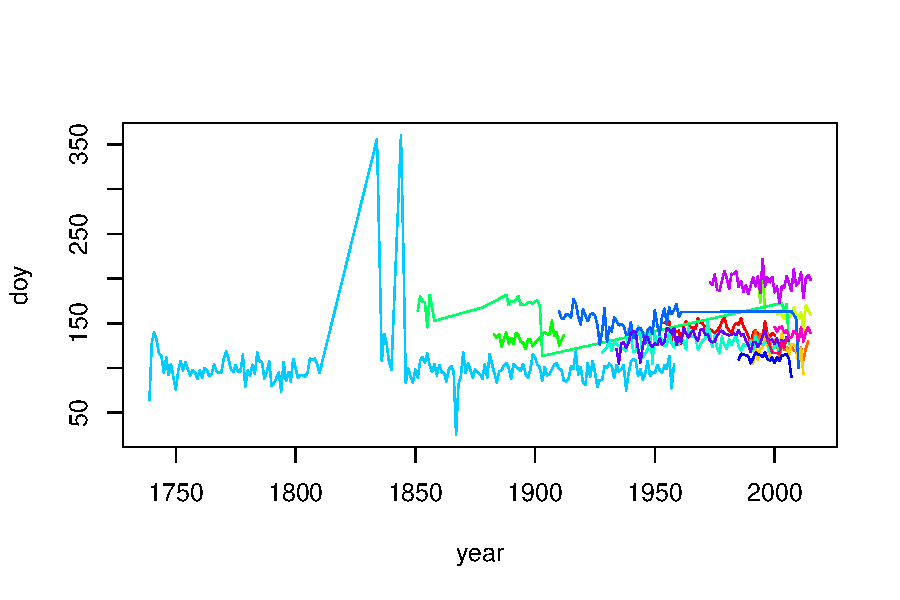
\includegraphics{meta_ep2_data-figobsdata}
\end{center}
\caption{Mean day of year (averaged across all events and species) by year from the observational data.}
\end{figure}

\subsection{Species}

\begin{Schunk}
\begin{Sinput}
> expdata$latbi <- paste(expdata$genus, expdata$species)
> obsdata$latbi <- paste(obsdata$genus, obsdata$species)
> length(expdata$latbi)
\end{Sinput}
\begin{Soutput}
[1] 64099
\end{Soutput}
\begin{Sinput}
> length(obsdata$latbi)
\end{Sinput}
\begin{Soutput}
[1] 211952
\end{Soutput}
\end{Schunk}

How many (and which species overlap between the two approaches?

\begin{Schunk}
\begin{Sinput}
> unique(expdata$latbi)[which(unique(expdata$latbi) %in% unique(obsdata$latbi))]
\end{Sinput}
\begin{Soutput}
 [1] "Acer rubrum"              "Carya tomentosa"          "Quercus alba"            
 [4] "Vaccinium pallidum"       "Vaccinium stamineum"      "Quercus rubra"           
 [7] "Chimaphila maculata"      "Hieracium venosum"        "Thalictrum thalictroides"
[10] "Betula lenta"             "Fagus grandifolia"        "Acer pensylvanicum"      
[13] "Castanea dentata"         "Viburnum lentago"         "Vaccinium corymbosum"    
[16] "Vaccinium vacillans"      "Prunus serotina"          "Viburnum acerifolium"    
[19] "Bromus hordeaceus"        "Geranium dissectum"       "Vicia sativa"            
[22] "Vulpia myuros"            "Pinus taeda"              "Nyssa sylvatica"         
[25] "Liquidambar styraciflua"  "Pinus strobus"            "Liriodendron tulipifera" 
[28] "Pinus virginiana"         "Fraxinus americana"       "Quercus velutina"        
[31] "Acer saccharum"           "Quercus phellos"          "Cornus florida"          
[34] "Juniperus virginiana"     "Diospyros virginiana"     "Betula alleghaniensis"   
[37] "Carya ovata"              "Ilex opaca"               "Quercus falcata"         
[40] "Quercus nigra"            "Carya glabra"             "Quercus stellata"        
[43] "Quercus coccinea"         "Magnolia virginiana"      "Cercis canadensis"       
[46] "Ulmus americana"          "Betula papyrifera"        "Prunus pensylvanica"     
[49] "Achillea millefolium"     "Andropogon gerardii"      "Erigeron strigosus"      
[52] "Panicum virgatum"         "Claytonia lanceolata"     "Campanula rotundifolia"  
[55] "Erythronium grandiflorum" "Eriogonum subalpinum"     "Ipomopsis aggregata"     
[58] "Lathyrus leucanthus"      "Amaranthus retroflexus"   "Setaria viridis"         
[61] "Lolium perenne"          
\end{Soutput}
\end{Schunk}

\end{document}
